\documentclass[unicode,12pt]{beamer}
\usetheme[progressbar=frametitle]{metropolis}    %プレゼンのテーマ設定

%if want to use pdfLatex, specify \iffalse to preamble for LuaLatex and XeLatex
%--------------- preamble for LuaLatex ------------------%

\iffalse
\usepackage{luatexja}
\usepackage[ipaex]{luatexja-preset}
\renewcommand{\kanjifamilydefault}{\gtdefault}
\setsansfont{Calibri}
\fi

%-----------------------------------------------------%

%--------------- preamble for XeLatex -------------------%

\iftrue
\usepackage{xltxtra}
\XeTeXlinebreaklocale "ja"
\usepackage{zxjatype}
\setCJKmainfont[]{Meiryo}
\setsansfont[Scale = 1.1]{Calibri}  % or Arial (Scale = 1)
\fi

%-----------------------------------------------------%

%--------------- general preamble -----------------------%

\definecolor{Cerulean blue}{rgb}{0.16, 0.32, 0.75}
\definecolor{darkcerulean}{rgb}{0.03, 0.27, 0.49}
\definecolor{skyblue}{rgb}{0.4, 0.6, 1.0}
\definecolor{lightpink}{rgb}{1.0, 0.8, 0.76}  %for block color
\definecolor{gray}{gray}{0.8}

\setbeamertemplate{blocks}[default] % Blockの影を消す
%\setbeamertemplate{items}[default] % 箇条書きをシンプルに
\setbeamertemplate{navigation symbols}{} % ナビゲーションシンボルを消す
\setbeamertemplate{footline}[frame number] % フッターはスライド番号のみ
\setbeamertemplate{itemize item}[circle]
\setbeamertemplate{itemize subitem}{--}
\setbeamercolor{frametitle}{bg=skyblue} %or Cerulean blue
\setbeamercolor{title}{fg=darkcerulean}

\iffalse
\usebackgroundtemplate{
    \includegraphics[width=\paperwidth,height=\paperheight]{beamer_background1.pdf}
}
\fi

\usepackage{color}


\newcommand{\emphasis}[2][red]{{\bf{\color{#1} #2}}}
\newcommand{\caveat}[2][blue]{{\bf{\color{#1} #2}}}
\newcommand{\fpartial}[3][\partial]{\frac{#1 #2}{#1 #3}}
\newcommand{\hpartial}[4][\partial]{\frac{#1^{#2} #3}{#1 #4^{#2}}}

\newcommand{\dlinecell}[1]{\begin{tabular}{@{}c@{}} #1 \end{tabular}}

\def\argmax{\text{arg} \max}
\def\argmin{\text{arg} \min}

%-----------------------------------------------------%

\title{Bunching to Maximize Tax Credits: Evidence from Kinks in the U.S. Tax Schedule}
\subtitle{Literature Review Workshop in 2020}
\author{Hiroki Kato}
\date{June 26, 2020}

\begin{document}

    \maketitle

    \section{Introduction}

    \begin{frame}
        \frametitle{Bunching}
    
        A growing field of public finance: bunching at kink points
        %
        \begin{itemize}
            \item A kink: an income amount for a given taxpayer at which marginal tax rates change discretely, marking the end of one tax bracket and the begging of the next.
        \end{itemize}
    
    \end{frame}

    \begin{frame}
        \frametitle{What This Paper Did}
    
        This paper investigates why bunching occurs at some kinks but not others,
        using several major tax acts.
        %
        \begin{itemize}
            \item These acts allow to observe changes in bunching patterns in response to changes in kink locations.
            \item Saez (2010) explains that some taxpayers may earn or report incomes to maximize refunds
            \item While Saez (2010) is unable to distinguish it from optimization frictions
            \item This paper can overcome this point and shows bunching is due to refund maximization.
        \end{itemize}
    
    \end{frame}

    \begin{frame}
        \frametitle{Contributions}
    
        \begin{enumerate}
            \item measures the overall extent of bunching at tax kinks in the U.S.;
            \item shows that many taxpayers gravitate towards the unique point of the tax schedule that maximizes the refund they receive.
            \item shows that bunching at refund-maximizing kinks is partly driven by persistence
            \item documents the emergence of bunching by war earners and shows that this is driven exclusively by income misreporting. 
        \end{enumerate}
    
    \end{frame}

    \begin{frame}
        \frametitle{Demonstration of Main Finding}
    
        \centerline{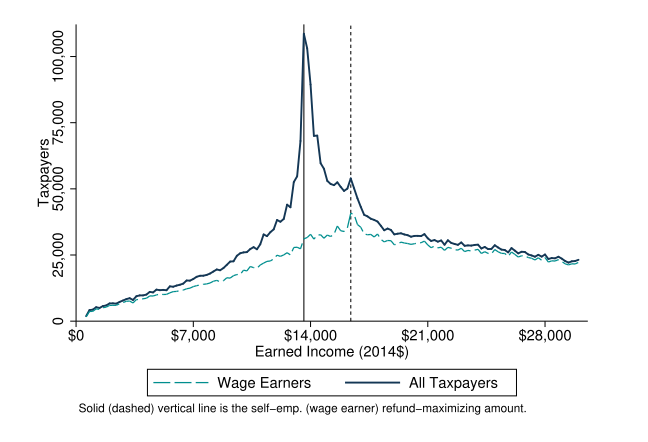
\includegraphics[width = \linewidth]{0626kato_fig/fig1.PNG}}
    
    \end{frame}
    

    \section{Data and Estimation}


    \begin{frame}
        \frametitle{Main Data}
    
        Panel data of 258 million tax returns that is representative of the tax-filing population in the United States
        in every year from 1996 to 2014.
        \begin{itemize}
            \item contain federal income tax returns (filed by taxpayers) and information returns (filed by third parties) of individuals
            \item Use information on date of birth and sex at the time of birth from the Social Security Administration's Data Master File.
            \item All data are pre-audit and therefore reflect what taxpayers report when filing, including any errors.
        \end{itemize}
    
    \end{frame}

    \begin{frame}
        \frametitle{Key issue of Bunching Estimation}
    
        How would taxpayers behave in the absence of a kink (counterfactual)?
        %
        \begin{itemize}
            \item Specify an alternative (local) tax schedule as well as the (local) distribution of income under the alternative tax schedule.
            \item Let $t_0$ denote the marginal tax rate that applies below a given kink $z^*$, and $t_1$ the rate that applies above it.
        \end{itemize}
    
    \end{frame}

    \begin{frame}
        \frametitle{Technique of Bunching Estimation}
    
        Chetty et al. (2011) estimates the counterfactual scenario in which $t_0$ applies both above and below $z^*$ with in a certain distance surrounding the kink (the "bunching region").
        %
        \begin{itemize}
            \item Note that this removes the kink within the region of study.
            \item To measure the amount of bunching ($\hat{B}$), compare the actual distribution of income with the predicted counterfactual distribution ($h_0$) of income under tax rate $t_0$.
        \end{itemize}
    
    \end{frame}

    \begin{frame}
        \frametitle{}
    
        Cont'd
        \begin{itemize}
            \item the counterfactual income distribution is predicted by observed data near kink but not so close as to be affected by bunching behavior (exclude the bins immediately surrounding the kink called "the bunching window").
            \item a bunching coefficient $\hat{b}$ is equal to the percentage of taxpayers inside the bunching window who are classified as bunchers. 
            \item standard errors for $\hat{B}$ and $\hat{b}$ are calculated by adding randomly sampled estimated residuals from the original regressions to the predicted values of the original regressions (bootstrap procedure).
        \end{itemize}
    
    \end{frame}

    \begin{frame}
        \frametitle{}
    
        \centerline{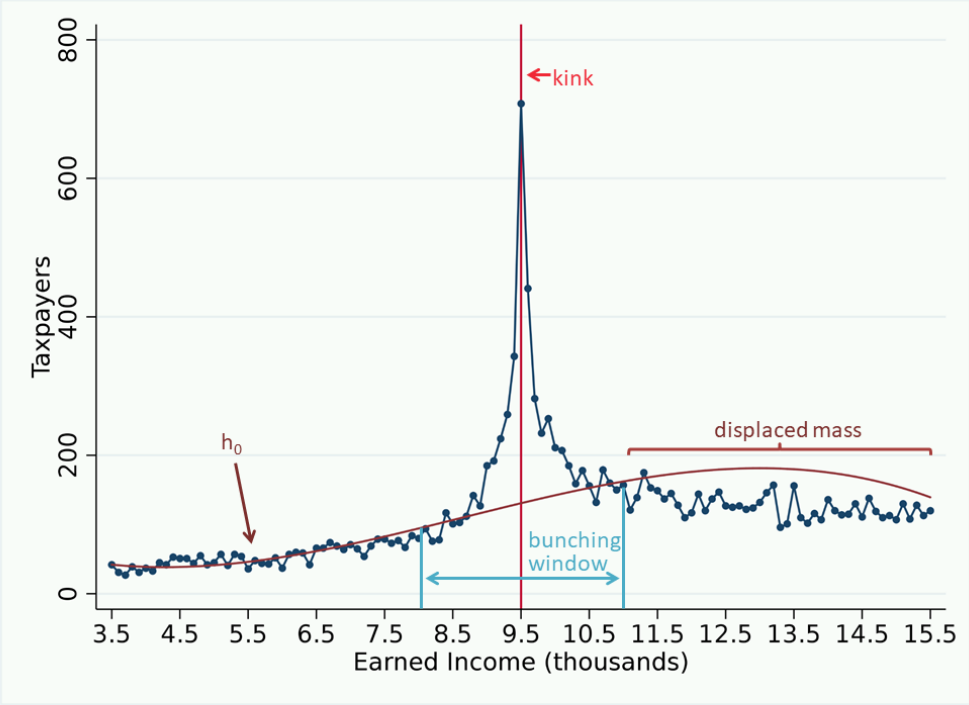
\includegraphics[width = \linewidth]{0626kato_fig/fig3.PNG}}
    
    \end{frame}

    \begin{frame}
        \frametitle{First Problem of Bunching Estimation}
    
        To impose integration constraint where the bunchers are reallocated.
        %
        \begin{itemize}
            \item this constraint reallocates them above the bunching window but within the bunching region (the total number of taxpayers within the bunching region is identical in the actual and counterfactual densities).
            \item In this context, some of mass should be reallocated outside of the bunching region (to the next higher kink), which leads to upper bias of $h_0$.
        \end{itemize}
    
    \end{frame}

    \begin{frame}
        \frametitle{Second Problem of Bunching Estimation}
    
        To remove the kink (the incentive to bunch) within region of study 
        %
        \begin{itemize}
            \item Suppose that we wish to analyze kink $K$, but kink $L$ lies somewhere inside $K$'s bunching window.
            \item This method may identify bunchers at kink $L$ as responding to kink $K$ (misattribution)
            \item To deal with this, they estimate the total number of bunchers in the usual way. and assign fraction $\Delta t_k/(\Delta t_K + \Delta t_L)$ to the bunchers to $K$, and one minus this fraction to$L$ where $\Delta t_j$ is marginal tax rates change at kink $j$.  
        \end{itemize}
    
    \end{frame}

    
    \section{Results}

    \begin{frame}
        \frametitle{Bunching at Refund Maximization?}
    
        \centerline{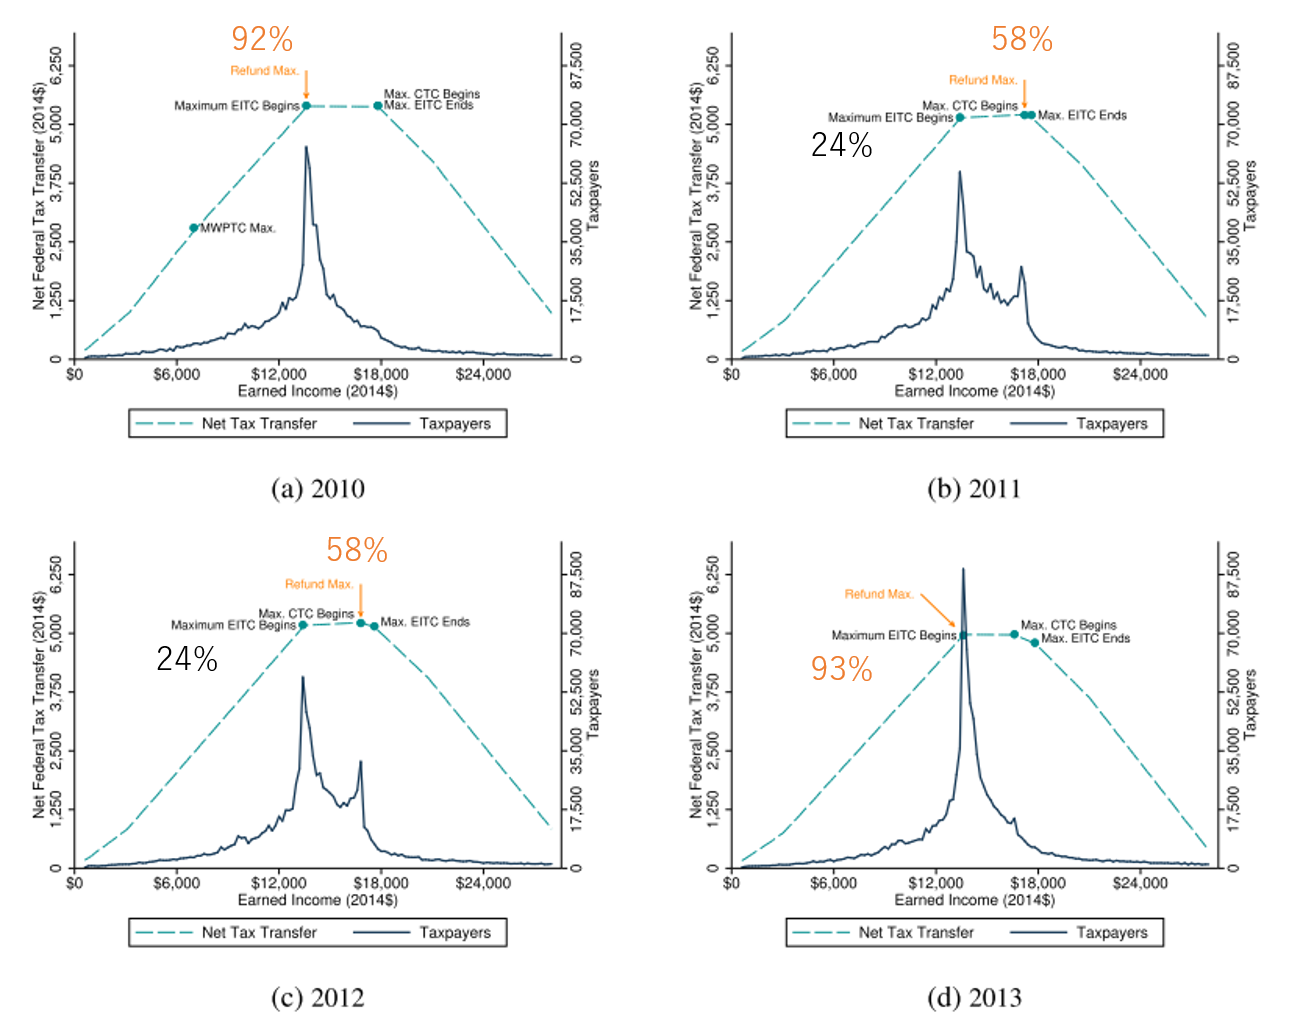
\includegraphics[width = 0.9\linewidth]{0626kato_fig/fig6_slide.PNG}}
    
    \end{frame}

    \begin{frame}
        \frametitle{Distort Economic Behavior? Noncompliance?}
    
        \centerline{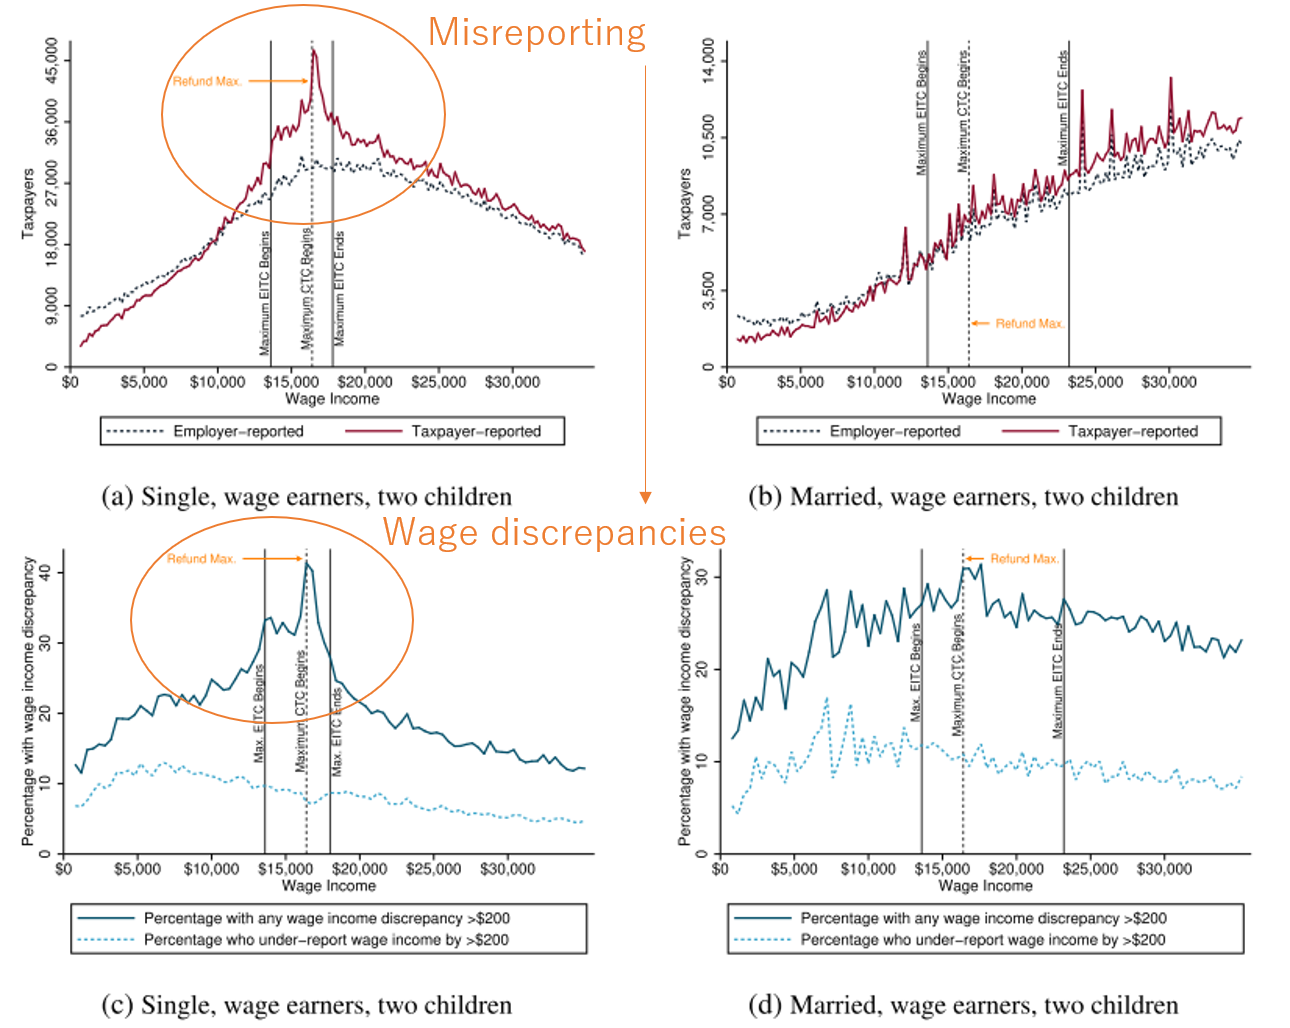
\includegraphics[width = 0.9\linewidth]{0626kato_fig/fig8_slide.png}}
    
    \end{frame}

    \begin{frame}
        \frametitle{Distort Economic Behavior? Noncompliance?}
    
        Remark: Probit regression to explore the characteristics of correlated with refund maximization
        %
        \begin{itemize}
            \item Motivation: Due to the incomplete nature of third-party reporting of self-employment earnings, an analogous exercises for the self-employed is not possible.
            \item Outcome: an indicator whether the taxpayer is within \$500 of their refund-maximizing kink.
            \item Result: Both wage earners and the self-employed are somewhat more likely to maximize refunds when no W-2 (employer-reported wage income) is present to substantiate wage income.
        \end{itemize}
    
    \end{frame}

    \begin{frame}
        \frametitle{Dynamics in Refund Maximization}
    
        \centerline{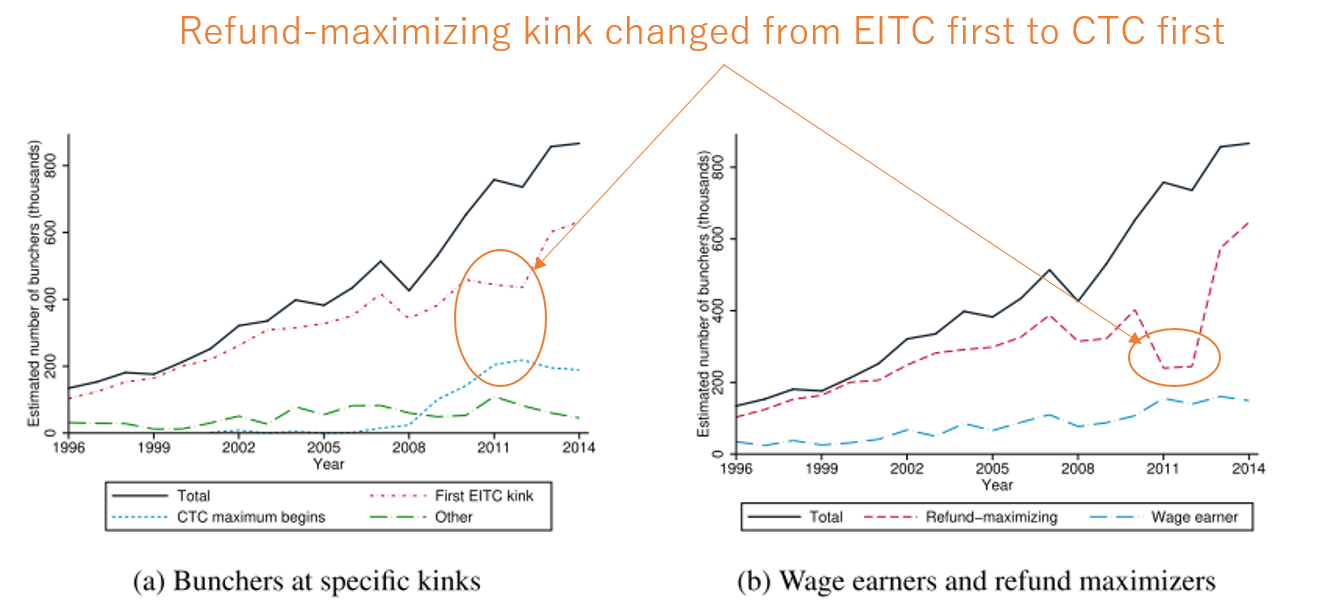
\includegraphics[width = \linewidth]{0626kato_fig/fig5_slide.png}}
    
    \end{frame}

    \begin{frame}
        \frametitle{Dynamics in Refund Maximization}
    
        \centerline{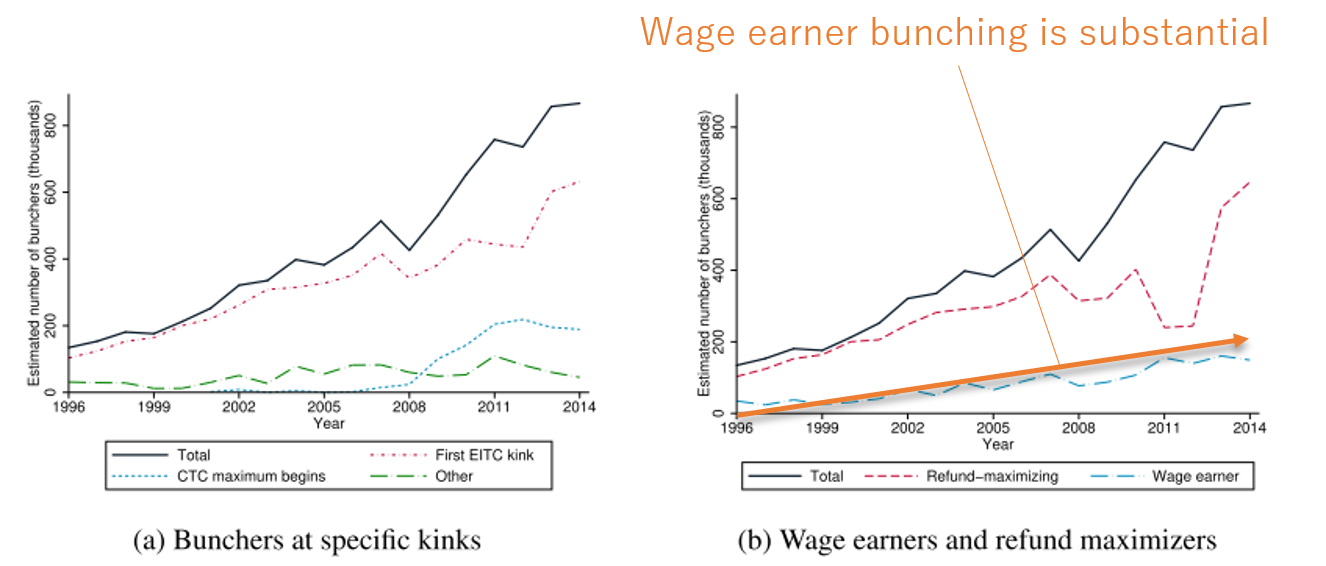
\includegraphics[width = \linewidth]{0626kato_fig/fig5_slide2.png}}
    
    \end{frame}

    \begin{frame}
        \frametitle{Tracking the new refund-maximizing kink}
    
        \centerline{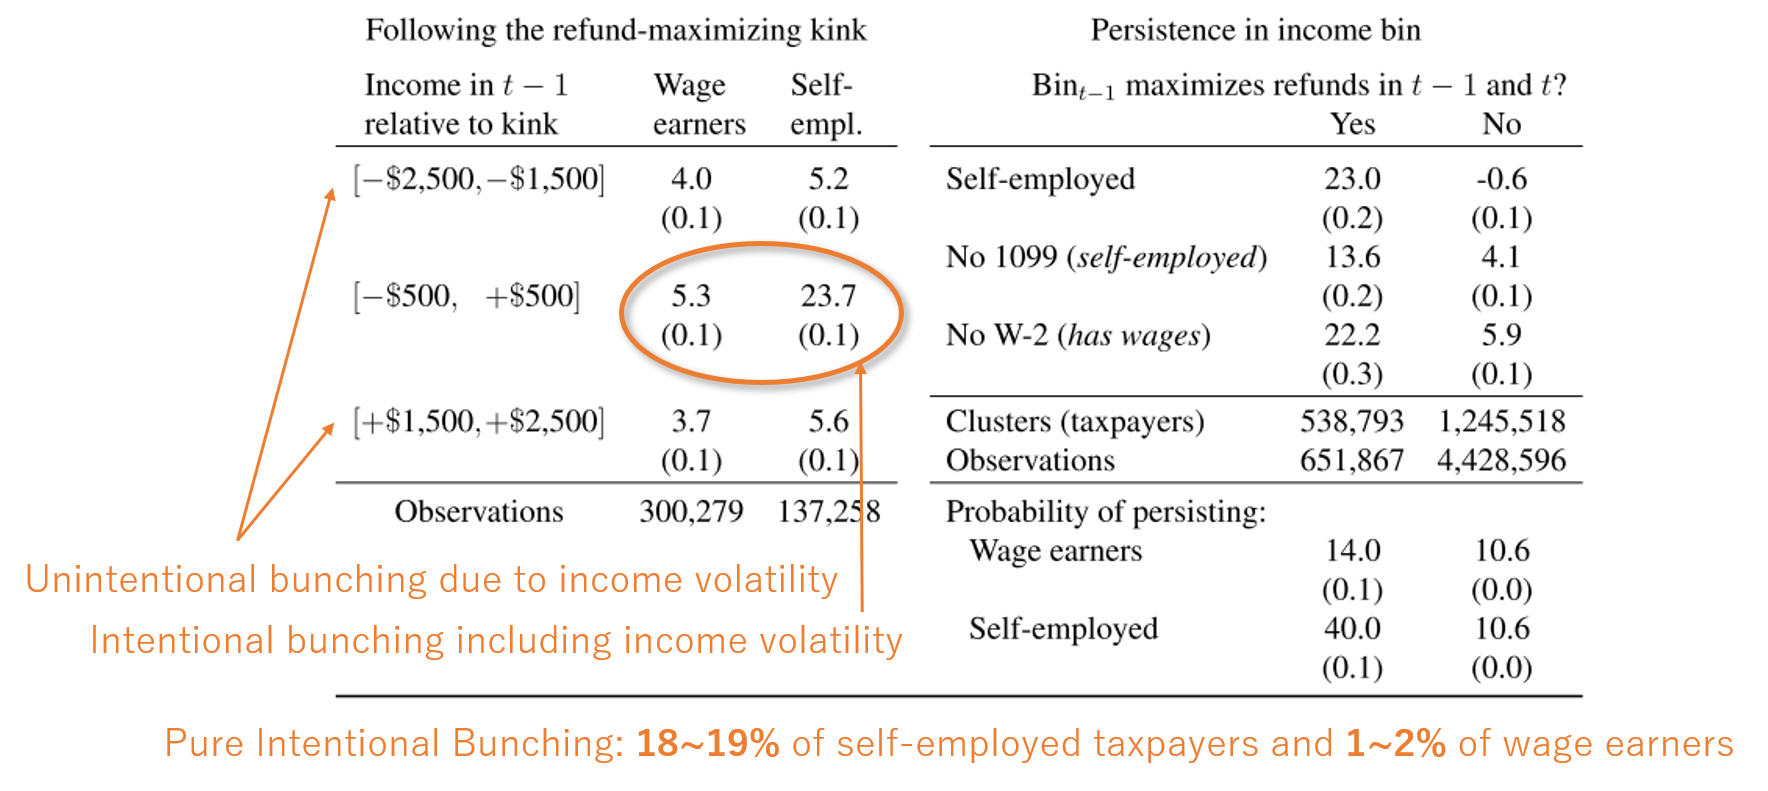
\includegraphics[width = \linewidth]{0626kato_fig/tab3_slide1.png}}
    
    \end{frame}

    \begin{frame}
        \frametitle{Remaining the same refund-maximizing kink}
    
        \centerline{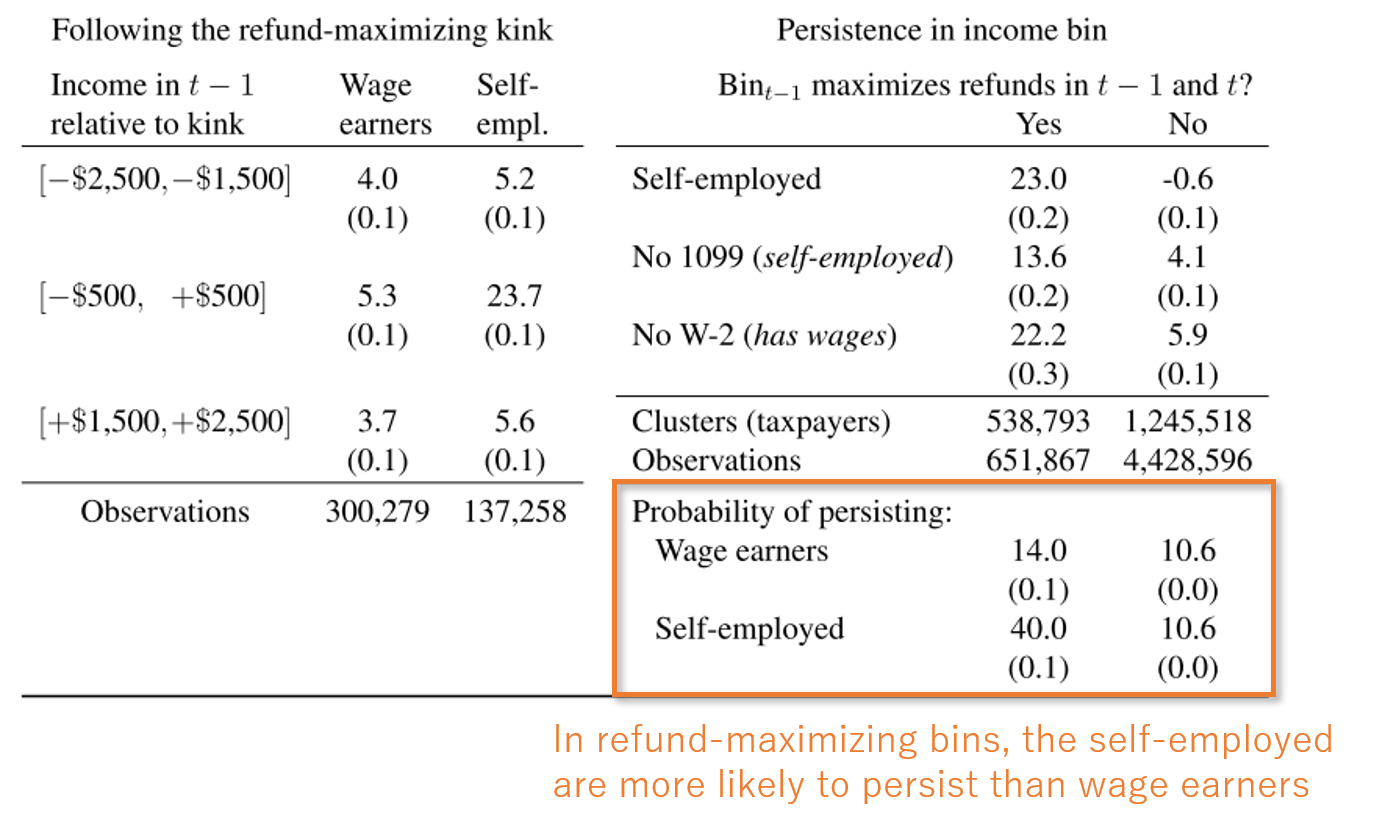
\includegraphics[width = \linewidth]{0626kato_fig/tab3_slide2.png}}
    
    \end{frame}

    
    \section{Concluding Remarks}

    \begin{frame}
        \frametitle{}
    
        \begin{quote}
            ..., we have uncovered several new facts about taxpayer bunching in the United States. Most notably, we have shown that bunching is particularly responsive at kinks that maximize taxpayer refunds. For many groups, when the refund-maximizing kink changes location between consecutive years, a large mass of taxpayers appears at the new refund-maximizing kink (Mortenson and Whitten, forthcoming, p.19). 
        \end{quote}
    
    \end{frame}


\end{document}